\documentclass[tikz, border=15pt]{standalone}
\usepackage{tikz}
\usetikzlibrary{calc, arrows.meta, positioning, shapes.geometric}

\definecolor{predictbg}{HTML}{EBF8FF}
\definecolor{predictborder}{HTML}{3182CE}
\definecolor{updatebg}{HTML}{F0FFF4}
\definecolor{updateborder}{HTML}{38A169}
\definecolor{measurebg}{HTML}{FFFAF0}
\definecolor{measureborder}{HTML}{DD6B20}
\definecolor{linecolor}{HTML}{2D3748}

\begin{document}
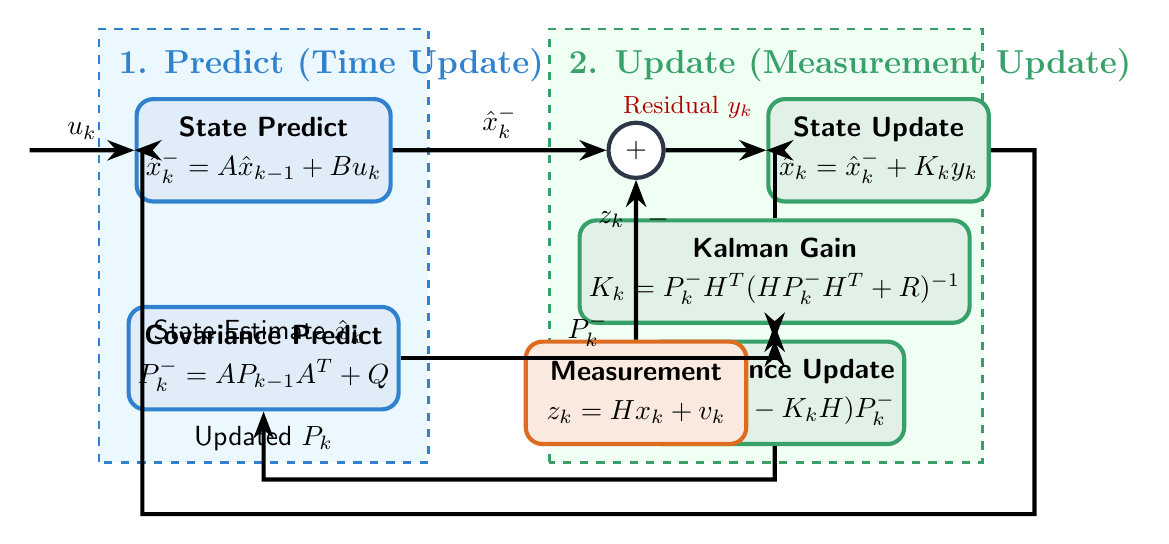
\begin{tikzpicture}[
    scale=1.1,
    >=Stealth,
    line width=1.2pt,
    font=\sffamily,
    block/.style={draw=#1, fill=#1!15, rounded corners=6pt, line width=1.5pt, minimum width=2.8cm, minimum height=1.3cm, align=center},
    sum/.style={draw=linecolor, circle, fill=white, line width=1.5pt, inner sep=0pt, minimum size=0.7cm}
]

    % Predict Step Container Box
    \fill[predictbg, draw=predictborder, dashed, line width=1pt] (-5.0, -1.8) rectangle (-1.2, 3.2);
    \node[predictborder, font=\bfseries\large, anchor=north west] at (-4.9, 3.1) {1. Predict (Time Update)};

    % Update Step Container Box
    \fill[updatebg, draw=updateborder, dashed, line width=1pt] (0.2, -1.8) rectangle (5.2, 3.2);
    \node[updateborder, font=\bfseries\large, anchor=north west] at (0.3, 3.1) {2. Update (Measurement Update)};

    % Nodes in Predict Step
    \node[block=predictborder] (state_pred) at (-3.1, 1.8) {\textbf{State Predict}\\[2pt]$\hat{x}_k^- = A \hat{x}_{k-1} + B u_k$};
    \node[block=predictborder] (cov_pred) at (-3.1, -0.6) {\textbf{Covariance Predict}\\[2pt]$P_k^- = A P_{k-1} A^T + Q$};

    % Nodes in Update Step
    \node[sum] (sum_res) at (1.2, 1.8) {$+$};
    \node[block=updateborder] (gain) at (2.8, 0.4) {\textbf{Kalman Gain}\\[2pt]$K_k = P_k^- H^T (H P_k^- H^T + R)^{-1}$};
    \node[block=updateborder] (state_upd) at (4.0, 1.8) {\textbf{State Update}\\[2pt]$\hat{x}_k = \hat{x}_k^- + K_k y_k$};
    \node[block=updateborder] (cov_upd) at (2.8, -1.0) {\textbf{Covariance Update}\\[2pt]$P_k = (I - K_k H) P_k^-$};

    % External Measurement Node
    \node[block=measureborder] (meas) at (1.2, -1.0) {\textbf{Measurement}\\[2pt]$z_k = H x_k + v_k$};

    % Flow Connections
    % Control Input
    \draw[->, line width=1.5pt] (-5.8, 1.8) -- (state_pred) node[midway, above] {$u_k$};

    % Predict to Sum & Gain
    \draw[->, line width=1.5pt] (state_pred) -- (sum_res) node[midway, above] {$\hat{x}_k^-$};
    \draw[->, line width=1.5pt] (sum_res) -- (state_upd) node[midway, above] {};
    \draw[->, line width=1.5pt] (cov_pred) -| (gain) node[near start, above] {$P_k^-$};
    \draw[->, line width=1.5pt] (cov_pred) -| (cov_upd);

    % Measurement & Residual
    \draw[->, line width=1.5pt] (meas) -- (sum_res) node[near end, left] {$z_k$} node[near end, right] {$-$};
    \node[font=\small, color=red!70!black] at (1.8, 2.3) {Residual $y_k$};

    % Gain to State & Covariance Update
    \draw[->, line width=1.5pt] (gain) |- (state_upd);
    \draw[->, line width=1.5pt] (gain) -- (cov_upd);

    % Feedback Loop back to Predict Step for k+1
    \draw[->, line width=1.5pt] (state_upd) -- (5.8, 1.8) -- (5.8, -2.4) -- (-4.5, -2.4) |- (state_pred) node[near start, right] {State Estimate $\hat{x}_k$};
    \draw[->, line width=1.5pt] (cov_upd) |- (2.8, -2.0) -- (-3.1, -2.0) -- (cov_pred) node[near start, above] {Updated $P_k$};

\end{tikzpicture}
\end{document}
